\documentclass[journal = jacsat, manuscript = article, layout = twocolumn]{achemso}

\usepackage[version = 4]{mhchem}
\usepackage{graphicx}
\usepackage{mwe}

% disable symbol next to email
\makeatletter
\def\acs@author@fnsymbol#1{}
\makeatother
% enable abstract
\AbstractOn
% put abstract and title on the same page
\let\oldmaketitle\maketitle
\let\maketitle\relax

% macros
\newcommand{\nidppe}{\ce{Ni(dppe)Cl2}}
\newcommand{\nicl}{\ce{NiCl2 $\cdot$ 6H2O}}
\newcommand{\nh}{\ce{NH3}}
\newcommand{\nanh}{\ce{Na $\cdot$ NH3}}
\newcommand{\nhbr}{\ce{NH4Br}}
\newcommand{\h}{$^1$H}
\newcommand{\p}{$^{31}$P}
\newcommand{\cdcl}{\ce{CDCl3}}
\newcommand{\del}{$\delta = $}
\newcommand{\niion}{\ce{Ni^{2+}}}
\newcommand{\wavenum}{cm$^{-1}$}

\title{1,2-bis(diphenylphosphino)ethane (dppe) and \nidppe\ synthesis via
solvated electron reduction}

\author{David Qiu}
\affiliation{Department of Chemistry, University of Illinois at
Urbana-Champaign, 505 S Matthews Avenue, Urbana, IL, 61801}
\email{davidlq2@illinois.edu}

\begin{document}

\twocolumn[
\begin{@twocolumnfalse}
\oldmaketitle
\hrule
\begin{abstract}

This experiment demonstrated successful synthesis of the dppe ligand via
solvated electron reduction of triphenylphosphine followed by treatment with
1,2-dichloroethane, as well as ligand substitution of \nicl\ to yield \nidppe.
The reaction had an overall yield of 117.74\% for dppe and 47\% for \nidppe. \h\
NMR, \p\ NMR, and IR spectra of dppe and \nidppe\ were analyzed, and confirmed
experimental success while noting the presence of excess solvent and residual
impurity. Future studies should improve upon this synthesis by minimizing
residual solvent, improving \nidppe\ yield via temperature control, and using
higher resolution NMR instruments to characterize dppe.

\end{abstract}
\hrule
\vspace{6mm}%
\end{@twocolumnfalse}
]

\section{Introduction}

\begin{figure}[H]
	
\includegraphics[width=0.5\textwidth]{figures/scheme.png}
	\caption*{Scheme 1: Synthesis of dppe via reduction of
	triphenylphosphine followed by reaction with 1,2-dichloroethane.}
\end{figure}

Ammonia is a versatile inorganic solvent with the unique property of dissolving
alkali metals to form solvated electrons, which act as extremely strong reducing
agents in solution. In this experiment, this property was used to reduce a
solution of triphenylphosphine to yield the bidentate ligand
1,2-bis(diphenylphosphino)ethane (dppe) upon reaction with 1,2-dichloroethane.
The dppe was used to perform ligand substitution on \nicl, generating its
corresponding complex \nidppe. This experiment demonstrates the efficacy of
cheap, readily-available reagents to synthesize useful coordinating ligands for
use in laboratory and industry.

\begin{figure}[H]
	
\includegraphics[width=0.4\textwidth]{figures/scheme-2.png}
	\caption*{Scheme 2: Synthesis of \nidppe\ via direct ligand substitution
	of \nicl.}
\end{figure}

\section{Results and Discussion}

The experiment resulted in a 117.74\% yield of dppe, and a 47\% yield of
\nidppe. Consequentially, the dppe was either not fully dry prior to NMR and IR
analysis, or it contained some residual impurity. The yield of \nidppe\ is
interesting as well, as it implies that the ligand substitution reaction (Scheme
2) was not driven to completion. This could be a result of either poor kinetics arising from reaction conditions (room temperature, short reaction time), or thermodynamic effects driving the reaction towards dissociation due to steric effects of the dppe ligand, though
this is unlikely as polydentate ligands are known to be highly stable \cite{textbook}.

To further investigate these findings, the 60 MHz \h\ and 400 MHz \p\ NMR
spectra taken in \cdcl\ were analyzed. The \h\ NMR spectrum of dppe was rather
poor; diethyl ether was a prominent impurity, and shifts corresponding to the
aromatic hydrogens were not discernible in the \h\ NMR spectra. These are due
both to the poor resolution of the 60 MHz instrument and the overlap with the
solvent \cdcl\ peak. This statement is supported by the integration of 20
aromatic protons underneath the broad peak \del\ 7.27 ppm, exactly corresponding
to the 20 aromatic protons of the 26 in dppe. This finding has been replicated
in other \h\ NMR spectra of dppe.\cite{dppenmr1}

\begin{figure}
	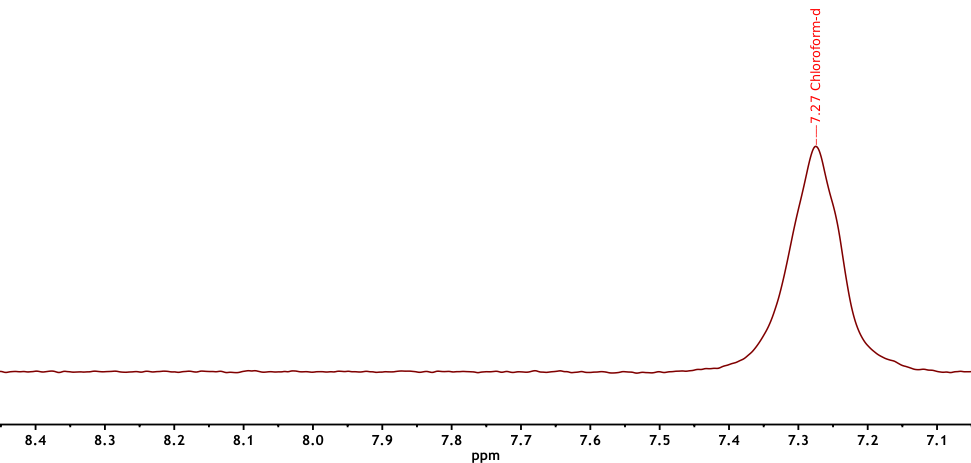
\includegraphics[width=0.4\textwidth]{figures/zoom_dppe_hnmr.png}
	\caption{\h\ NMR of dppe, magnified to highlight the aromatic shifts at
	\del\ 7.27 ppm (20 H). Note the overlap with the existing \cdcl\ peak and
the diethyl ether signal (\del\ 3.68 ppm, q).}

	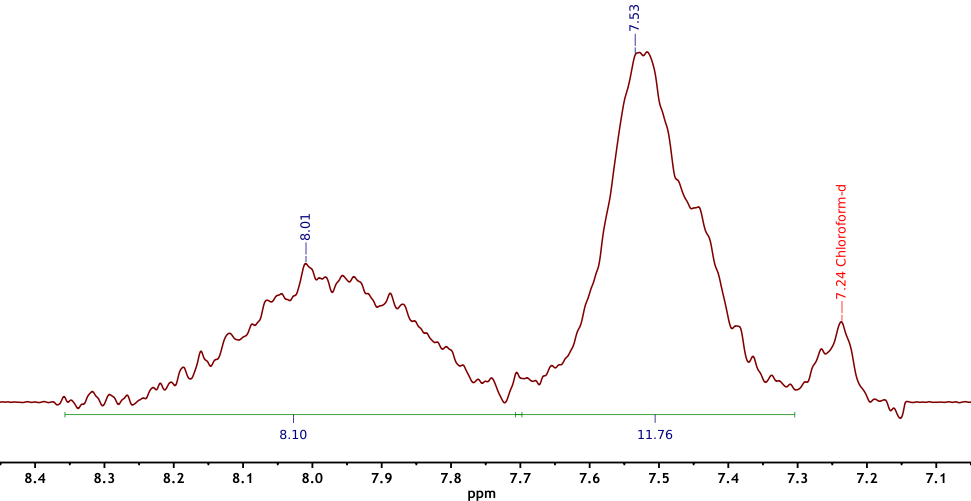
\includegraphics[width=0.4\textwidth]{figures/zoom_nidppe_hnmr.png}
	\caption{\h\ NMR of dppe, magnified to highlight the aromatic shifts at
	\del\ 8.01 ppm (16 H) and \del\ 7.53 (24 H). Note the distinguished
\cdcl\ peak (\del\ 7.24 ppm) upon formation of the nickel complex.}
\end{figure}

This hypothesis is further supported by the \h\ NMR spectrum of \nidppe, which was
able to distinguish the same aromatic protons from the \cdcl\ shift. This is
because the presence of the \niion\ metal center withdraws electron density from
the lone pairs of phosphorus and the aromatic protons, causing them to appear
further downfield and distinguishing the protons meta to phosphorus from those
that are ortho or para to phosphorus.

The \p\ NMR spectra were not particularly revealing, as there exists only one
chemically distinct phosphorus atom in both dppe and \nidppe. However, there was
an unknown impurity at \del\ -105.91 ppm and \del\ -221.00 ppm observed in both
\p\ NMR spectra. This finding was not replicated elsewhere, suggesting that its
corresponding impurities are unique to this synthetic method or the materials
used in this experiment.

Aside from the aforementioned impurities and the \h\ NMR multiplicities
(indistinguishable due to the poor resolution), the chemical shifts of both the
\h\ and \p\ spectra are in good agreement with existing studies done on dppe and
\nidppe.\cite{dppenmr1, dppenmr2}

The IR spectrum of dppe was not noteworthy, and indicated exclusively a C-H
stretch and an O-H impurity. Interestingly, the IR spectrum of \nidppe\ was
completely absent in the 3000-4000 \wavenum\ region. This is in fact largely
consistent with existing IR studies on \nidppe\cite{dppeir}, which indicate
exceedingly weak C-H stretches in \nidppe.

In conclusion, this experiment demonstrated the successful synthesis of the dppe
ligand via solvated electron reduction of triphenylphosphine followed by
treatment with 1,2-dichloroethane, as well as ligand substitution to yield
\nidppe. As indicated by the \h\ NMR, \p\ NMR, and IR analysis, future studies
should improve upon this synthesis by minimizing residual solvent, improving
\nidppe\ yield via temperature control, and using higher resolution NMR
instruments to characterize dppe.

\section{Experimental Procedures}

\textbf{dppe synthesis\cite{handout}:} To a round bottom flask was charged 200
mL of \nh, a glass-coated stir bar, and a dry ice condenser. Na (2.379 g, 0.1035
mol, 4 equiv.) was added slowly over 3 minutes. A dark blue solution was allowed
to form over 10 minutes, and then triphenylphosphine (13.55 g, 0.05166 mol, 2
equiv.) was added in 1 g portions.  This solution reacted for 30 minutes, after
which \nhbr\ (5.068 g, 0.05174 mol, 2 equiv.) was added. 1,2-dichloroethane
(2.555 g, 0.02582 mol, 1 equiv.) was poured in and reacted for 10 minutes.  The
flask was left open to air for 1 week.

The dried dppe was washed with DI water and rotary evaporated following
dilution with ethanol. The purified dppe crystals then precipitated, and were
filtered out of solution and washed with ethanol.

\textbf{\nidppe\ synthesis\cite{handout}:} \nicl\ (0.320 g, 1.34 mol, 1 equiv.)
was dissolved in ethanol and mixed with dppe (0.54 g, 1.34 mol, 1 equiv.). This
was allowed to react for 5 minutes, forming a tomato-red solution.  \nidppe\ was
filtered out and washed with diethyl ether. \h, \p\ NMR and IR spectra were
taken of dppe and \nidppe, and are available for viewing in the Supporting
Information.

\bibliography{lab_3.bib}

\end{document}
